\documentclass{article}
\usepackage[paperwidth=360pt,paperheight=230pt,margin=0pt,noheadfoot]{geometry}
\usepackage{tikz}
\usetikzlibrary{calc}

\definecolor{ink}{RGB}{28,41,56}
\definecolor{axis}{RGB}{100,116,139}
\definecolor{grid}{RGB}{203,213,225}
\definecolor{curve}{RGB}{30,64,175}
\definecolor{teal}{RGB}{13,148,136}
\definecolor{tealfill}{RGB}{176,227,219}
% Integral diagrams use exactly one semantic palette: blue for the
% lower-only part, yellow for the upper-only (or still unresolved) part, and
% green for their common part.  The common part is explicit rather than an
% alpha blend, so the three meanings stay distinct after GIF quantization.
\definecolor{blue}{RGB}{0,114,178}
\definecolor{bluefill}{RGB}{86,180,233}
\definecolor{yellow}{RGB}{230,159,0}
\definecolor{yellowfill}{RGB}{255,218,102}
\definecolor{green}{RGB}{0,128,84}
\definecolor{greenfill}{RGB}{89,190,142}
\definecolor{orange}{RGB}{234,88,12}
\definecolor{orangefill}{RGB}{254,215,170}
\definecolor{purple}{RGB}{126,34,206}
\definecolor{yellowedge}{RGB}{202,138,4}
\definecolor{projection}{RGB}{148,163,184}
\colorlet{under}{blue}
\colorlet{underfill}{bluefill}
\colorlet{over}{yellow}
\colorlet{overfill}{yellowfill}
\colorlet{shared}{green}
\colorlet{sharedfill}{greenfill}
\colorlet{gap}{yellow}
\colorlet{gapfill}{yellowfill}

\pagestyle{empty}
\setlength\parindent{0pt}
\setlength\topskip{0pt}
\begin{document}
\noindent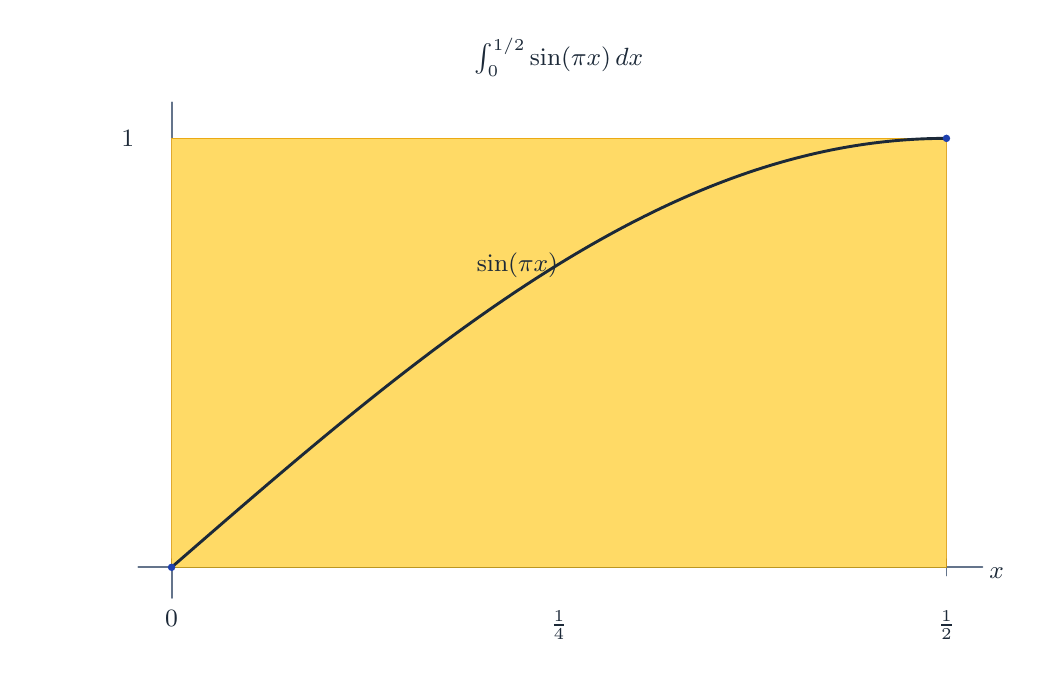
\begin{tikzpicture}[baseline=(current bounding box.north),x=1pt,y=1pt,line cap=round,line join=round]
\useasboundingbox (0,0) rectangle (360,230);
\draw[axis,line width=.75pt] (40,35) -- (345,35);
\draw[axis,line width=.75pt] (52,24) -- (52,203);
\draw[grid,line width=.3pt] (52,35) -- (52,190);
\draw[axis,line width=.55pt] (52,32) -- (52,38);
\draw[grid,line width=.3pt] (332,35) -- (332,190);
\draw[axis,line width=.55pt] (332,32) -- (332,38);
\path[fill=sharedfill] (52,35) rectangle (332,35);
\path[fill=overfill] (52,35) rectangle (332,190);
\draw[under,draw opacity=.8,line width=0.45pt] (52,35) rectangle (332,35);
\draw[over,draw opacity=.8,line width=0.45pt] (52,35) rectangle (332,190);
\draw[ink,line width=1.05pt] plot[smooth] coordinates {(52,35) (53.8667,36.6231) (55.7333,38.2461) (57.6,39.8687) (59.4667,41.4907) (61.3333,43.1121) (63.2,44.7325) (65.0667,46.3519) (66.9333,47.9701) (68.8,49.5868) (70.6667,51.2019) (72.5333,52.8153) (74.4,54.4267) (76.2667,56.0359) (78.1333,57.6429) (80,59.2473) (81.8667,60.8492) (83.7333,62.4481) (85.6,64.0441) (87.4667,65.6369) (89.3333,67.2263) (91.2,68.8122) (93.0667,70.3944) (94.9333,71.9727) (96.8,73.5469) (98.6667,75.117) (100.5333,76.6826) (102.4,78.2436) (104.2667,79.7999) (106.1333,81.3513) (108,82.8976) (109.8667,84.4387) (111.7333,85.9743) (113.6,87.5044) (115.4667,89.0287) (117.3333,90.547) (119.2,92.0593) (121.0667,93.5653) (122.9333,95.0649) (124.8,96.5579) (126.6667,98.0442) (128.5333,99.5235) (130.4,100.9958) (132.2667,102.4608) (134.1333,103.9185) (136,105.3685) (137.8667,106.8109) (139.7333,108.2454) (141.6,109.6718) (143.4667,111.0901) (145.3333,112.5) (147.2,113.9014) (149.0667,115.2942) (150.9333,116.6781) (152.8,118.0532) (154.6667,119.4191) (156.5333,120.7757) (158.4,122.1229) (160.2667,123.4606) (162.1333,124.7886) (164,126.1067) (165.8667,127.4149) (167.7333,128.7129) (169.6,130.0006) (171.4667,131.2779) (173.3333,132.5447) (175.2,133.8007) (177.0667,135.0459) (178.9333,136.2802) (180.8,137.5033) (182.6667,138.7152) (184.5333,139.9158) (186.4,141.1048) (188.2667,142.2822) (190.1333,143.4478) (192,144.6016) (193.8667,145.7433) (195.7333,146.8728) (197.6,147.9901) (199.4667,149.095) (201.3333,150.1874) (203.2,151.2672) (205.0667,152.3342) (206.9333,153.3884) (208.8,154.4296) (210.6667,155.4576) (212.5333,156.4725) (214.4,157.474) (216.2667,158.4621) (218.1333,159.4367) (220,160.3976) (221.8667,161.3448) (223.7333,162.2781) (225.6,163.1975) (227.4667,164.1028) (229.3333,164.9939) (231.2,165.8708) (233.0667,166.7334) (234.9333,167.5815) (236.8,168.415) (238.6667,169.2339) (240.5333,170.0381) (242.4,170.8275) (244.2667,171.602) (246.1333,172.3616) (248,173.106) (249.8667,173.8353) (251.7333,174.5494) (253.6,175.2482) (255.4667,175.9316) (257.3333,176.5995) (259.2,177.252) (261.0667,177.8888) (262.9333,178.5099) (264.8,179.1154) (266.6667,179.705) (268.5333,180.2787) (270.4,180.8365) (272.2667,181.3783) (274.1333,181.9041) (276,182.4138) (277.8667,182.9073) (279.7333,183.3845) (281.6,183.8455) (283.4667,184.2902) (285.3333,184.7185) (287.2,185.1304) (289.0667,185.5258) (290.9333,185.9047) (292.8,186.2671) (294.6667,186.6129) (296.5333,186.942) (298.4,187.2545) (300.2667,187.5503) (302.1333,187.8294) (304,188.0917) (305.8667,188.3372) (307.7333,188.5659) (309.6,188.7778) (311.4667,188.9728) (313.3333,189.1509) (315.2,189.3121) (317.0667,189.4564) (318.9333,189.5837) (320.8,189.6941) (322.6667,189.7876) (324.5333,189.864) (326.4,189.9235) (328.2667,189.966) (330.1333,189.9915) (332,190)};
\fill[curve] (52,35) circle[radius=1.35pt];
\fill[curve] (332,190) circle[radius=1.35pt];
\node[font=\small,text=ink,anchor=north] at (52,23) {$0$};
\node[font=\small,text=ink,anchor=north] at (192,23) {$\frac14$};
\node[font=\small,text=ink,anchor=north] at (332,23) {$\frac12$};
\node[font=\small,text=ink,anchor=east] at (42,190) {$1$};
\node[font=\small,text=ink,anchor=west] at (344,33) {$x$};
\node[font=\small,text=ink] at (177,144) {$\sin(\pi x)$};
\node[font=\small,text=ink,anchor=south] at (192,209) {$\int_0^{1/2}\sin(\pi x)\,dx$};
\end{tikzpicture}
\end{document}
